% chap6.tex - Week 6
\cleardoublepage
%\phantomsection
\chapter{Week 6}

\section{Day 1 - ``My private little stash''}
\subsection{Getting interrrupted}

We're getting close to the point where we can really start using Git as we originally intended, the team at Tamagoyaki Inc. are also getting much more acquainted with the operations of both version control and Git in particular.  Unfortunately things don't always go as smoothly as we would like.  The following scenario demonstrates just this.

\begin{trenches}
``Yeh but Martha, I need you to work on this fix now!  Not in five minutes.''

``Klaus I'm kinda in the middle of something else yet, and I'm not ready to commit,'' said Martha, feeling a little concerned.  She was used to Klaus making demands on his time, but she had spent a while working on this particular fix for John and she just wasn't ready to finish up yet.

``You could always use the stash feature.''  It was Rob again, it seemed as if this young user had cottoned on to Git quicker than most of the seasoned developers.''

Klaus seemed unimpressed, ``What the heck does that do?''

``Allows you to move your changes to somewhere else until you are ready to finish them.''

``Please Rob,'' started Martha, ``Can you show me what you mean?  Sounds exactly like what I need''
\end{trenches}

Sometimes you could be in the middle of something when another really important task comes up.  When this happens you are often required to drop everything and carry on with another task.  Often this can be quite difficult.  You may be in a development branch, but unable or unwilling to make a commit at this stage.  So how can we deal with this?

Well, one way of dealing with this situation, and this is not necessarily the best way, is to do the steps outlined below;

\begin{enumerate}
\item Make a new branch called something like WIP
\item Pull changes into this new branch
\item Commit changes into WIP branch
\item Switch back to the branch we need to work on
\item Make our changes and commit them
\item Merge in our WIP branch on top with the \texttt{--no-commit} option
\item Delete the WIP branch
\item Continue development in our original branch
\end{enumerate}

That may seem like a lot of work.  OK, the benefit is a fairly awesome one, but at the cost of considerable command line hackery to get there.  It would be nice if there was an easy way to do the above, and though someone of you may be screaming something like \emph{shell script} right about now, you can rest your fingers.  We actually have another tool in the Git toolbox to help us out.

The \texttt{git stash} command is used for exactly these situations.  Let us make a quick example of how to use it in our test repository.  To begin with we are going to make a few changes to the \textbf{master} branch, before we are interrupted.

\begin{Verbatim}[frame=leftline,framerule=1mm,fontsize=\relsize{-3}] 
john@satsuki:~/coderepo$ git checkout master
Already on 'master'
john@satsuki:~/coderepo$ echo "Number strings rule 1234" >> 
 another_file
john@satsuki:~/coderepo$ 
\end{Verbatim}

So now we are interrupted and we have to make some important, and urgent changes to our \textbf{master} branch.  The example that follows is one way that we could use the \texttt{git stash} command to help us out.  

\begin{Verbatim}[frame=leftline,framerule=1mm,fontsize=\relsize{-3}] 
john@satsuki:~/coderepo$ git stash
Saved working directory and index state WIP on master: d50ffb2 Merged 
 in zaney
HEAD is now at d50ffb2 Merged in zaney
john@satsuki:~/coderepo$ echo "Some mega important changes" >> newfile1
john@satsuki:~/coderepo$ git commit -a -m 'Important Update'
[master 9cb2af2] Important Update
 1 files changed, 1 insertions(+), 0 deletions(-)
john@satsuki:~/coderepo$ 
\end{Verbatim}

So using the \texttt{git stash} command, we have squirrelled all of our developmental changes away into a \emph{stash}.  Now we have completed the mega important change that just could not wait, we are ready to pull our changes back from the stash.  First let us see just what the stash contains.

\begin{Verbatim}[frame=leftline,framerule=1mm,fontsize=\relsize{-3}] 
john@satsuki:~/coderepo$ git stash list
stash@{0}: WIP on master: d50ffb2 Merged in zaney
john@satsuki:~/coderepo$ git stash show stash@{0}
 another_file |    1 +
 1 files changed, 1 insertions(+), 0 deletions(-)
john@satsuki:~/coderepo$ git stash show stash@{0} -p
diff --git a/another_file b/another_file
index dba885d..b3a5cc5 100644
--- a/another_file
+++ b/another_file
@@ -1 +1,2 @@
 New stuff
+Number strings rule 1234
john@satsuki:~/coderepo$ 
\end{Verbatim}

As you can see, the \texttt{-p} option to the \texttt{git stash show} command shows us exactly what is contained in the stash.  We can apply this stash by running the following;

\begin{Verbatim}[frame=leftline,framerule=1mm,fontsize=\relsize{-3}] 
john@satsuki:~/coderepo$ git stash apply stash@{0}
# On branch master
# Changed but not updated:
#   (use "git add <file>..." to update what will be committed)
#   (use "git checkout -- <file>..." to discard changes in working 
 directory)
#
#	modified:   another_file
#
# Untracked files:
#   (use "git add <file>..." to include in what will be committed)
#
#	my_third_committed_file
#	temp_file
no changes added to commit (use "git add" and/or "git commit -a")
john@satsuki:~/coderepo$ git commit -a -m 'Continued Development'
[master 37950f8] Continued Development
 1 files changed, 1 insertions(+), 0 deletions(-)
john@satsuki:~/coderepo$ git stash list
stash@{0}: WIP on master: d50ffb2 Merged in zaney
john@satsuki:~/coderepo$ 
\end{Verbatim}

Our stash has been applied to the current branch, in our case \textbf{master}, and we have gone ahead and committed these changes into the repository.  In this case we didn't have anything else to add to the index before we went ahead and committed it.  

Interestingly though, our stash still exists.  If we had used the \texttt{git stash pop} command instead of the \texttt{git stash apply}, our stash would have been removed.  Of course we can have multiple stashes in our repository.  For completeness sake, let us learn how to manually remove a stash, and take a look at how our repository looks with our semi-graphical \texttt{git log}

\begin{Verbatim}[frame=leftline,framerule=1mm,fontsize=\relsize{-3}] 
john@satsuki:~/coderepo$ git stash drop stash@{0}
Dropped stash@{0} (193f27172fc0df278105b981815c7718204030d8)
john@satsuki:~/coderepo$ git log --graph --pretty=oneline --all 
 --abbrev-commit --decorate
* 37950f8 (HEAD, master) Continued Development
* 9cb2af2 Important Update
*   d50ffb2 Merged in zaney
|\  
| * 7cc32db (zaney) Made another awesome change
| * a27d49e Made an awesome change
* | ed2301b Removed third file
* |   b119573 Merge branch 'wonderful'
|\ \  
| * | cfbecab (wonderful) Fantastic new feature
| |/  
* | 4ac9201 Updated third file
|/  
* 9710177 Added another file
* 55fb69f (v2.0) Added two new files
* 4a155e4 Removed a few files
* a022d4d (tag: v1.0b, v1.0a) Messed with a few files
* 9938a0c Finished adding initial files
* 163f061 (v0.9) Made a few changes to first and second files
* cfe23cb My First Ever Commit
john@satsuki:~/coderepo$ 
\end{Verbatim}

So using the \texttt{git stash drop} command, you can see that it is fairly simple to drop a single stash from the list.


\section{Day 2 - ``What?! No backup?''}
\subsection{Attack of the clones}

We now know about basic branching and merging.  At this stage, there is on important topic we must cover briefly, and this is subject of cloning.  Cloning allows you to make a complete copy of your repository, including all of its history and all of the branches.  Let us take a look at a situation which could make use of cloning.

\begin{trenches}
``So John,'' started Rob, ``Just how are we backing up the repository at the moment?''

John thought for a moment before replying.  He knew what Rob was getting at, but he hadn't expected Rob to bring the question up in front of Markus.  In truth he had forgotten all about it.  He turned to Markus.

``I'll be honest Markus.  Currently the repository isn't being backed up, but then we are running in parallel with the old system, so it wouldn't be the end of the world if we lost it.''

Markus nodded and smiled.  It seemed that John had gotten away with it for now and with that, Klaus shot Rob a piercing glance.  

``Team,'' began Markus, ``we need a definitive way of backing up the new Git repository, and I'd like it done before the end of the day.''  He pointed at a document on the table.  ``This project document has been approved by Wayne, and in there it states we will have a defined backup strategy.  Please don't let me down.''

\begin{center} * * * \end{center}

``Rob you really got to be careful about things like that,'' Klaus said to one of the younger members of the team.  ``You really showed John up in there.''  

``Yeh,'' said Rob, ``I realise that now.''  He stood with his back against the wall and tapped his fingers against the painted surface.  ``I was wondering, do you think John would let me look at the backup system for him as a way of apologising.''

Klaus smiled, it seemed Rob was finally understanding things, ``Go ask him,'' said Klaus, ``He's so snowed under with the BurnForce release that he'll probably let you implement it too''

``Right'' nodded Rob and off he went.
\end{trenches}

So cloning is an excellent way of taking a copy of our repository, in essence it is a simple way of taking a backup of our repository and then with a little more work, we can keep that clone up to date.  Obviously we could just take the files and copy them, but a better way of doing this is by utilising the \texttt{git clone} command.  When cloning a repository, we take then entire structure and replicate it, creating an exact copy of the data in an alternative location.  Well, that's what cloning means isn't it?

The git clone tool doesn't just copy the data though, it does several other things.  Let us create a clone of our test repository to another local location.  In this case, we are going to clone the repository into a folder called \texttt{coderepo-cl}.

\begin{Verbatim}[frame=leftline,framerule=1mm,fontsize=\relsize{-3}] 
john@satsuki:~$ git clone coderepo coderepo-cl
Initialized empty Git repository in /home/john/coderepo-cl/.git/
john@satsuki:~$ 
\end{Verbatim}

\begin{Verbatim}[frame=leftline,framerule=1mm,fontsize=\relsize{-3}] 
john@satsuki:~$ cd coderepo-cl
john@satsuki:~/coderepo-cl$ ls 
another_file  newfile1  newfile2
john@satsuki:~/coderepo-cl$
\end{Verbatim}

\begin{Verbatim}[frame=leftline,framerule=1mm,fontsize=\relsize{-3}] 
john@satsuki:~/coderepo-cl$ git status
# On branch master
nothing to commit (working directory clean)
john@satsuki:~/coderepo-cl$ 
\end{Verbatim}

Let us take a few moments to see what has happened here.  It would appear that our data has been copied successfully.  If you were to run a \texttt{git log} on this dir, you would see all the previous log messages for all our previous commits.  You can also see that if we run \texttt{git status} that we are on the same branch here that we were in our repository when we left it.  In this case, we are in the \textbf{master} branch.

So this could be sufficient enough to serve as a backup of our repository, but we will actually find a better way to do this a little later.

\section{Day 3 - ``Is this clone for real?''}
\subsection{Not entirely as expected}

We now have a clone of the repository and we can start to look at how we can play with branches and see how the two are different.

\begin{trenches}
``Klaus, this doesn't make sense though.  I cloned my repo, but my branches have vanished,'' started Rob, rather worriedly.

``I'm sure they haven't gone anywhere,'' shouted John.  

Rob's reply was quick and certain, ``They have!  Run a git branch on your clone and see for yourself''

``Oh!''

Rob smiled the smug smile of a man who is pleased he was right.

\begin{center} * * * \end{center}

``Rob?'' asked John tentatively, aware of his previous state of anguish.

His reply indicated a less than stressed demeanour, ``Sup, dude?''.

John was pleasantly surprised, ``Did you sort out the branch issue?''

Rob began walking over to John, ``Yeh, try running git branch with the r parameter.''

\end{trenches}

You may be thinking that we now have a detached copy of the other branches in our repository.  That's not exactly accurate.  Let us run the command that Rob suggested and see what is happening.  

\begin{Verbatim}[frame=leftline,framerule=1mm,fontsize=\relsize{-3}] 
john@satsuki:~/coderepo-cl$ git branch
* master
john@satsuki:~/coderepo-cl$ git branch -r
  origin/HEAD -> origin/master
  origin/master
  origin/wonderful
  origin/zaney
john@satsuki:~/coderepo-cl$ 
\end{Verbatim}

Whilst we have all the objects in our repository, we do not yet have our branches set up locally.  They are available, but they have not yet been setup locally.  To explain this we need to introduce the concept of remote tracking branches.  We are familiar with local branches.  Local branches allowed us to make commits locally in a safe and separated environment.  Remote tracking branches are links to remote branches which allow us to track the development of that branch and bring it in to a local one if we so desire.

Let us take a look at what we can do with these remote tracking branches.  Notice in the output above, we have the word \texttt{origin} in front of the branch names.  When we clone a repository, Git automatically sets up what is called a \emph{remote}.  We can view this by using the \texttt{git remote} tool.

\begin{Verbatim}[frame=leftline,framerule=1mm,fontsize=\relsize{-3}] 
john@satsuki:~/coderepo-cl$ git remote
origin
john@satsuki:~/coderepo-cl$ git remote -v
origin	/home/john/coderepo (fetch)
origin	/home/john/coderepo (push)
john@satsuki:~/coderepo-cl$ 
\end{Verbatim}

As you can see from the output above, the \textbf{origin} remote definition points to the original folder that our repository came from.  So now we know that when referring to \texttt{origin/master}, we are really talking about the \textbf{master} branch which is located at the remote location \textbf{origin}.

We are going to spend a little while now learning about remote branches and how they differ to local branches.  Let us spend a few minutes trying some of our normal operations against a remote branch.  The first operation we are going to try is a diff.  We are going to run a diff between our current \textbf{master} branch and the \textbf{wonderful} branch as it stands in the original repository, so we should be diffing between \texttt{master} and \texttt{origin/wonderful}.  For brevity, we are also going to limit the changes shown to those which affect \texttt{newfile1} only, by appending \texttt{ -- <filename>} to the command.

\begin{Verbatim}[frame=leftline,framerule=1mm,fontsize=\relsize{-3}] 
john@satsuki:~/coderepo-cl$ git diff master origin/wonderful -- 
 newfile1
diff --git a/newfile1 b/newfile1
index f32a0e6..ef20984 100644
--- a/newfile1
+++ b/newfile1
@@ -1,3 +1,2 @@
 A new file
-and some more awesome changes
-Some mega important changes
+and some more changes
john@satsuki:~/coderepo-cl$ 
\end{Verbatim}

So we can see that our diff command completed successfully.  Note that this command requires no connection to our \textbf{origin} repository, as all of the data has been cloned locally, more on this later.  

Let us run another command now and learn a little more about what the remote reference \textbf{origin} really means.

\begin{Verbatim}[frame=leftline,framerule=1mm,fontsize=\relsize{-3}] 
john@satsuki:~/coderepo-cl$ git remote show origin
* remote origin
  Fetch URL: /home/john/coderepo
  Push  URL: /home/john/coderepo
  HEAD branch: master
  Remote branches:
    master    tracked
    wonderful tracked
    zaney     tracked
  Local branch configured for 'git pull':
    master merges with remote master
  Local ref configured for 'git push':
    master pushes to master (up to date)
john@satsuki:~/coderepo-cl$ 
\end{Verbatim}

Though this command introduces some terms that we are not yet familiar with yet, like push, pull and fetch, we can see that the \textbf{origin} remote has been set up to \emph{track} three branches called, \textbf{master}, \textbf{wonderful} and \textbf{zaney}.  So although these branches are not yet usable in the way a local branch would be, it is comforting to know that Git does know about them.  Let us continue playing with the remote branch and run a \texttt{git log} command against it.

\begin{Verbatim}[frame=leftline,framerule=1mm,fontsize=\relsize{-3}] 
john@satsuki:~/coderepo-cl$ git log origin/master -- newfile1
commit 9cb2af2a00fd2253060e6bf8cc6c377b3d55ecea
Author: John Haskins <john.haskins@tamagoyakiinc.koala>
Date:   Tue Apr 19 16:43:59 2011 +0100

    Important Update

commit d50ffb2fa536d869f2c4e89e8d6a48e0a29c5cc1
Merge: ed2301b 7cc32db
Author: John Haskins <john.haskins@tamagoyakiinc.koala>
Date:   Fri Apr 1 07:42:04 2011 +0100

    Merged in zaney

...
...
...
\end{Verbatim}

Again, this requires no connection to the \textbf{origin} repository at all and works as expected.  Let us try something really funky now, let us try checking out a remote branch so that we can view the filesystem.  We are now going to try checking out the remote branch called \textbf{wonderful}.

\begin{Verbatim}[frame=leftline,framerule=1mm,fontsize=\relsize{-3}] 
john@satsuki:~/coderepo-cl$ git checkout origin/wonderful
Note: checking out 'origin/wonderful'.

You are in 'detached HEAD' state. You can look around, make 
experimental changes and commit them, and you can discard any 
commits you make in this state without impacting any branches 
by performing another checkout.

If you want to create a new branch to retain commits you create, you 
may do so (now or later) by using -b with the checkout command again. 
Example:

  git checkout -b new_branch_name

HEAD is now at cfbecab... Fantastic new feature
john@satsuki:~/coderepo-cl$ 
\end{Verbatim}

Interesting.  This is not what we are used to seeing.  When we have checked out branches before, we have always been presented with a \texttt{Switched to branch 'xxxxxx'} message.  Now we are seeing a funny message about having a detatched HEAD.  This is because we are not actually on a branch.  We can make changes as we are advised, we can even make commits, but these will not actually become integrated into any branches.  In essence these commits would be left dangling and after time, because no branch points to them, they would get deleted by garbage collection routines.

Running the \texttt{git branch} command below confirms our suspicions.

\begin{Verbatim}[frame=leftline,framerule=1mm,fontsize=\relsize{-3}] 
john@satsuki:~/coderepo-cl$ git branch -v
* (no branch) cfbecab Fantastic new feature
  master      37950f8 Continued Development
john@satsuki:~/coderepo-cl$ 
\end{Verbatim}

So we really need to figure out how to make these branches exist locally so that we can commit to them and retain those commits.  To do this we use the \texttt{git branch} tool again, but we use it in a slightly different manner.  

\begin{Verbatim}[frame=leftline,framerule=1mm,fontsize=\relsize{-3}] 
john@satsuki:~/coderepo-cl$ git checkout -b wonderful origin/wonderful 
Branch wonderful set up to track remote branch wonderful from origin.
Switched to a new branch 'wonderful'
john@satsuki:~/coderepo-cl$ 
\end{Verbatim}

We are now on a local instance of the \textbf{wonderful} branch.  Let us take a minute to understand what that means.  As Git is a distributed environment, our local \textbf{wonderful} branch, is not going to be synchronised with the remote end automatically.  It would require effort on our part.  What this does mean though, is that we are able to begin committing to this branch and experimenting with it.

\section{Day 4 - ``Help I'm no longer up to date?''}
\subsection{Pulling changes, not teeth}

With a remote tracking branch, we can pull in the changes from the remote repository.  In our case, the remote repository is in the \texttt{coderepo} directory that we created at the start of the book.  In the \texttt{coderepo-cl} directory we have a separate, self-contained copy of the repository.  At the moment, because no changes have occurred to either, they contain exactly the same data.

By running the \texttt{git remote} tool again, we can see which branches are set up locally to track their remote counterparts in \textbf{origin}.

\begin{Verbatim}[frame=leftline,framerule=1mm,fontsize=\relsize{-3}] 
john@satsuki:~/coderepo-cl$ git remote show origin
* remote origin
  Fetch URL: /home/john/coderepo
  Push  URL: /home/john/coderepo
  HEAD branch: master
  Remote branches:
    master    tracked
    wonderful tracked
    zaney     tracked
  Local branches configured for 'git pull':
    master    merges with remote master
    wonderful merges with remote wonderful
  Local refs configured for 'git push':
    master    pushes to master    (up to date)
    wonderful pushes to wonderful (up to date)
john@satsuki:~/coderepo-cl$ 
\end{Verbatim}

What we are going to do now is make some changes to our original repository and see how we can view those changes and indeed pull them into our current local working repository, or clone.  Note that in the following code examples we have switched back to working on our original repository, in the \texttt{coderepo} folder.

\begin{Verbatim}[frame=leftline,framerule=1mm,fontsize=\relsize{-3}] 
john@satsuki:~/coderepo-cl$ cd ../coderepo
john@satsuki:~/coderepo$ git branch
* master
  wonderful
  zaney
john@satsuki:~/coderepo$ git checkout wonderful 
Switched to branch 'wonderful'
john@satsuki:~/coderepo$ git merge master
Updating cfbecab..37950f8
Fast-forward
 another_file            |    1 +
 my_third_committed_file |    1 -
 newfile1                |    3 ++-
 newfile2                |    2 +-
 4 files changed, 4 insertions(+), 3 deletions(-)
 delete mode 100644 my_third_committed_file
john@satsuki:~/coderepo$ echo "These changes are in the origin" >> 
 newfile3
john@satsuki:~/coderepo$ git add newfile3
john@satsuki:~/coderepo$ git commit -a -m 'Added a new file'
[wonderful 1c3206a] Added a new file
 1 files changed, 1 insertions(+), 0 deletions(-)
 create mode 100644 newfile3
john@satsuki:~/coderepo$ 
\end{Verbatim}

As you can see, we have switched back to working on our old \textbf{orgin} and have bought \textbf{wonderful} to be in line with master and have added a new file and committed the changes.  Now let us go back to our clone and see if we can see those changes.

\begin{Verbatim}[frame=leftline,framerule=1mm,fontsize=\relsize{-3}] 
john@satsuki:~/coderepo$ cd ../coderepo-cl/
john@satsuki:~/coderepo-cl$ git diff wonderful origin/
origin/HEAD        origin/master      origin/wonderful   origin/zaney 
john@satsuki:~/coderepo-cl$ git diff wonderful origin/wonderful 
john@satsuki:~/coderepo-cl$ 
\end{Verbatim}

That seems a little odd at first glance.  We have tried to view a diff between our local \textbf{wonderful} branch and the remote \textbf{origin/wonderful} branch.  Interestingly, Git is telling us that there is no difference.  Hang on though, we just made some changes above.  

Remember before we discussed the fact that our clone was disconnected from the \textbf{origin} copy?  What this means is that unless we ask Git, it won't update details about what is present in the remote copy.  Once this is up to date, we can pull the changes into our local copy of the remote branch?  Interestingly there are actually two ways to do this.

The first method is by running a \texttt{git pull} command.  If you remember the output from the \texttt{git remote show origin}, you may remember that it showed that there was a local branch configured for \texttt{'git pull'} and the details it gave for the \textbf{wonderful} branch were as follows; \texttt{wonderful merges with remote wonderful}.  What this means, is that when we run a \texttt{git pull} from inside the \textbf{wonderful} branch, Git will automatically contact the remote repository, update the list of changes and merge them into the local branch if possible.

We mentioned that there were two methods to perform the procedure.  Whilst the first one is to use \texttt{git pull}, the second one actually achieves an almost identical result, but by running two commands instead of one.  In point of fact, these two commands are executed by the \texttt{git pull} command.  Running them as two separate commands allows us to understand a little more about what is happening.  Let us run the command and then explain what we have done.

\begin{Verbatim}[frame=leftline,framerule=1mm,fontsize=\relsize{-3}] 
john@satsuki:~/coderepo-cl$ git fetch origin
remote: Counting objects: 4, done.
remote: Compressing objects: 100% (2/2), done.
remote: Total 3 (delta 1), reused 0 (delta 0)
Unpacking objects: 100% (3/3), done.
From /home/john/coderepo
   cfbecab..1c3206a  wonderful  -> origin/wonderful
john@satsuki:~/coderepo-cl$ git diff wonderful origin/wonderful 
diff --git a/another_file b/another_file
index dba885d..b3a5cc5 100644
--- a/another_file
+++ b/another_file
@@ -1 +1,2 @@
 New stuff
+Number strings rule 1234
...
...
...

john@satsuki:~/coderepo-cl$ git merge origin/wonderful 
Updating cfbecab..1c3206a
Fast-forward
 another_file            |    1 +
 my_third_committed_file |    1 -
 newfile1                |    3 ++-
 newfile2                |    2 +-
 newfile3                |    1 +
 5 files changed, 5 insertions(+), 3 deletions(-)
 delete mode 100644 my_third_committed_file
 create mode 100644 newfile3
john@satsuki:~/coderepo-cl$ 
\end{Verbatim}

As you can see, the two commands that we used were \texttt{git fetch} and the more familiar \texttt{git merge}.  The \texttt{git fetch} command literally visits the remote repository, in our case we asked for \textbf{origin}, and finds which objects are new.  These are then copied to the local clone, and the HEADs of the various remote branches are updated.  We now rerun our \texttt{git diff}, only this time, we see a great many more changes than before.  Finally we initiate a \texttt{git merge} to pull the changes from the now up to date remote branch to our local one.

We could have used the \texttt{git pull} command here, and if we had supplied no parameters to it, it would have achieved the exact same outcome.  The only difference would have been running one command instead of two.  Please note, that there are occasions when you would require one over the other, but as an introduction, this should be sufficient.

\section{Day 5 - ``I'm putting my foot down''}
\subsection{Pushing back!}

We now know a lot about remote locations right?  We are ready to start collaborating with someone.  Let us first see how Tamagoyaki are getting on with things.

\begin{trenches}
``But I know I have the remote right Simon, it's giving some weird error about refusing to update it.''  Rob was getting more than a little cross now.  

``Maybe you got the command wrong?'' asked Simon.

Rob slammed his hands down on the keyboard, ``Well then you come over here and type it, but I don't understand how hard it is to write git push.''  He shook his head, ``I even checked using the git remote tool and the push is apparently all set up.''

``Are you trying to push to a non-bare repository?'' Chirped Klaus.  He had been listening to the discussion escalate from mild annoyance to key shattering intrusion.  ``You can't push to a non-bare repository, else everything gets out of sync.''

``What do you mean bare?'' asked Rob.

Klaus smiled and his head appeared over the cubicle.  ``Come over here genius and I'll show you,'' he said with the slightest amount of gloat at being one of the only people to know something about Git that Rob didn't.
\end{trenches}

Bare?  Non-bare?  At first glance, this may seem confusing.  It isn't exactly an intuitive word to describe a repository but what Klaus mentioned was absolutely true.  In Git, if you want to push changes back to a repository, instead of pulling them, the repository that you push to should be what is called a \emph{bare} repository.  What this means is that the repository has no working copy.

\begin{figure}[hbt]
\tikzstyle{mybox} = [draw=black, fill=gray!20, very thick, rectangle, rounded corners, inner sep=15pt, inner ysep=20pt]
\tikzstyle{fancytitle} =[fill=black, text=white]
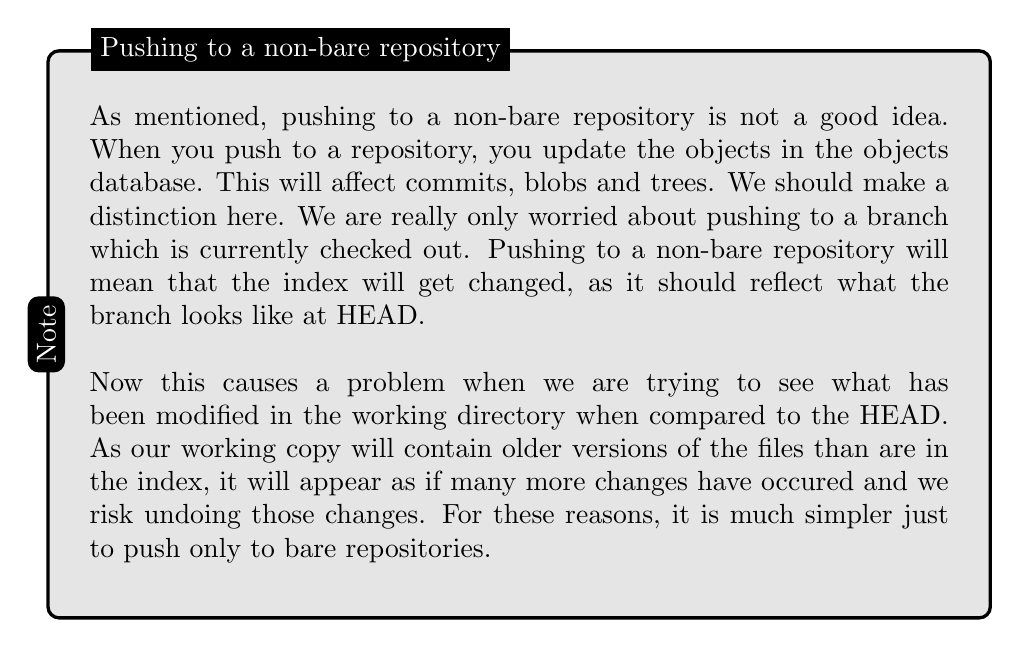
\begin{tikzpicture}
\node [mybox] (box){%
    \begin{minipage}{.9\textwidth}
As mentioned, pushing to a non-bare repository is not a good idea.  When you push to a repository, you update the objects in the objects database.  This will affect commits, blobs and trees.  We should make a distinction here.  We are really only worried about pushing to a branch which is currently checked out.  Pushing to a non-bare repository will mean that the index will get changed, as it should reflect what the branch looks like at HEAD.  
\newline
\newline
Now this causes a problem when we are trying to see what has been modified in the working directory when compared to the HEAD.  As our working copy will contain older versions of the files than are in the index, it will appear as if many more changes have occured and we risk undoing those changes.  For these reasons, it is much simpler just to push only to bare repositories.
    \end{minipage}
};
\node[fancytitle, right=16pt] at (box.north west) {Pushing to a non-bare repository};
\node[fancytitle, rounded corners] at (box.west) {\rotatebox{90}{Note}};
\end{tikzpicture}
\end{figure}

At first glance this may seem like a rather odd thing to want.  Why would we want a repository that doesn't have a working tree?  The simple answer is that a \emph{bare} repository allows us to be able to push changes into it.  Let us recreate the error message that Rob was talking about.

\begin{Verbatim}[frame=leftline,framerule=1mm,fontsize=\relsize{-3}] 
john@satsuki:~/coderepo-cl$ echo "This is another update to newfile3" 
 >> newfile3
john@satsuki:~/coderepo-cl$ git commit -a -m 'Added more to newfile3'
[wonderful dbf1e9a] Added more to newfile3
 1 files changed, 1 insertions(+), 0 deletions(-)
\end{Verbatim}

We have made a modification to the \textbf{wonderful} branch.  So let us now try to push that back to the \textbf{origin} remote repository with the \texttt{git push} command.
 
\begin{Verbatim}[frame=leftline,framerule=1mm,fontsize=\relsize{-3}] 
john@satsuki:~/coderepo-cl$ git push
Counting objects: 5, done.
Compressing objects: 100% (3/3), done.
Writing objects: 100% (3/3), 335 bytes, done.
Total 3 (delta 1), reused 0 (delta 0)
Unpacking objects: 100% (3/3), done.
remote: error: refusing to update checked out branch: 
 refs/heads/wonderful
remote: error: By default, updating the current branch in a non-bare 
remote: error: repository is denied, because it will make the index 
remote: error: and work tree inconsistent with what you pushed, and 
remote: error: will require 'git reset --hard' to match the work 
remote: error: tree to HEAD.
remote: error: 
remote: error: You can set 'receive.denyCurrentBranch' configuration 
remote: error: variable to 'ignore' or 'warn' in the remote repository 
remote: error: to allow pushing into its current branch; however, this 
remote: error: is not recommended unless you arranged to update its 
remote: error: work tree to match what you pushed in some other way.
remote: error: 
remote: error: To squelch this message and still keep the default 
remote: error: behaviour, set 'receive.denyCurrentBranch' configuration 
remote: error: variable to 'refuse'.
To /home/john/coderepo
 ! [remote rejected] wonderful -> wonderful (branch is currently checked out)
error: failed to push some refs to '/home/john/coderepo'
john@satsuki:~/coderepo-cl$ 
\end{Verbatim}

Bingo!  There is the error we were looking for.  In order to get round this, we are going to create another clone of the repository in \texttt{coderepo}.  This time however, we are going to pass an option to it when we create it.

\begin{Verbatim}[frame=leftline,framerule=1mm,fontsize=\relsize{-3}] 
john@satsuki:~/coderepo-cl$ cd ..
john@satsuki:~$ git clone coderepo coderepo-bk --bare
Initialized empty Git repository in /home/john/coderepo-bk/
john@satsuki:~$ cd coderepo-bk/
john@satsuki:~/coderepo-bk$ ls
branches  config  description  HEAD  hooks  info  objects  
packed-refs  refs
john@satsuki:~/coderepo-bk$ cd ..
john@satsuki:~$ cd coderepo-cl/
john@satsuki:~/coderepo-cl$ 
\end{Verbatim}

As you can see, creating the clone with the \texttt{--bare} option has had a definite effect on the structure of the clone itself.  In fact, the contents of the \texttt{coderepo-bk} folder look remarkably similar to the \texttt{.git} folder found in our normal working tree.  They are in fact, one and the same.  We have removed the need for a separate \texttt{.git} folder because we do not require a working tree.  Therefore, the contents of the \texttt{.git} folder and placed in the root \texttt{coderepo-bk} folder.

We are getting closer to making our push.  We have created a \emph{bare} repository, which we should now be able to push to.  The problem is, we have not yet defined our new repository as a remote location in the \texttt{coderepo-cl} repository.  This is something we will do now and to do this, we will use our \texttt{git remote} tool once more, this time employing the \texttt{add} parameter.

\begin{Verbatim}[frame=leftline,framerule=1mm,fontsize=\relsize{-3}] 
john@satsuki:~/coderepo-cl$ git remote add backup 
 /home/john/coderepo-bk
john@satsuki:~/coderepo-cl$ git remote show backup
* remote backup
  Fetch URL: /home/john/coderepo-bk
  Push  URL: /home/john/coderepo-bk
  HEAD branch: wonderful
  Remote branches:
    master    new (next fetch will store in remotes/backup)
    wonderful new (next fetch will store in remotes/backup)
    zaney     new (next fetch will store in remotes/backup)
  Local refs configured for 'git push':
    master    pushes to master    (up to date)
    wonderful pushes to wonderful (fast-forwardable)
john@satsuki:~/coderepo-cl$ 
\end{Verbatim}

We have created a remote called backup.  As you can see, some interrogation of the remote repository has taken place.  It is already aware of the branches present in our remote location.  Let us do a \texttt{git fetch} to update the local references.

\begin{Verbatim}[frame=leftline,framerule=1mm,fontsize=\relsize{-3}] 
john@satsuki:~/coderepo-cl$ git fetch backup
From /home/john/coderepo-bk
 * [new branch]      master     -> backup/master
 * [new branch]      wonderful  -> backup/wonderful
 * [new branch]      zaney      -> backup/zaney
john@satsuki:~/coderepo-cl$ git remote show backup
* remote backup
  Fetch URL: /home/john/coderepo-bk
  Push  URL: /home/john/coderepo-bk
  HEAD branch: wonderful
  Remote branches:
    master    tracked
    wonderful tracked
    zaney     tracked
  Local refs configured for 'git push':
    master    pushes to master    (up to date)
    wonderful pushes to wonderful (fast-forwardable)
john@satsuki:~/coderepo-cl$ 
\end{Verbatim}

Now we can see that all of the remote references for our \textbf{backup} remote have been updated.  If we run a diff against our local \textbf{wonderful} branch and the remote branch \textbf{backup/wonderful}, we can see the differences.

\begin{Verbatim}[frame=leftline,framerule=1mm,fontsize=\relsize{-3}] 
john@satsuki:~/coderepo-cl$ git diff wonderful backup/wonderful 
diff --git a/newfile3 b/newfile3
index 7268b97..638113c 100644
--- a/newfile3
+++ b/newfile3
@@ -1,2 +1 @@
 These changes are in the origin
-This is another update to newfile3
john@satsuki:~/coderepo-cl$ git branch -v
\end{Verbatim}

There we go!  Those are the changes we just committed to the local repository.  The last thing we need to do is to initiate a \texttt{git push}.  We are going to have to define which remote we wish to push to now for two reasons.  The first is that now we have two remotes, and so Git would not know if we meant \textbf{origin} or \textbf{backup}.  The second reason is that by default, the \textbf{wonderful} branch is set up to push to the \textbf{origin} remote.

\begin{Verbatim}[frame=leftline,framerule=1mm,fontsize=\relsize{-3}] 
john@satsuki:~/coderepo-cl$ git push backup
Counting objects: 5, done.
Compressing objects: 100% (3/3), done.
Writing objects: 100% (3/3), 335 bytes, done.
Total 3 (delta 1), reused 0 (delta 0)
Unpacking objects: 100% (3/3), done.
To /home/john/coderepo-bk
   1c3206a..dbf1e9a  wonderful -> wonderful
john@satsuki:~/coderepo-cl$ 
\end{Verbatim}

There we go, we have now managed to push our changes to a remote location.  In this case, we have pushed an update from the \textbf{wonderful} branch to the \textbf{backup/wonderful branch}.  If we wanted to, we could have pushed our repository to a new branch name, or indeed any of the existing branch names.

\begin{Verbatim}[frame=leftline,framerule=1mm,fontsize=\relsize{-3}] 
john@satsuki:~/coderepo-cl$ git push backup wonderful:newbranch
Total 0 (delta 0), reused 0 (delta 0)
To /home/john/coderepo-bk
 * [new branch]      wonderful -> newbranch
john@satsuki:~/coderepo-cl$ git remote show backup
* remote backup
  Fetch URL: /home/john/coderepo-bk
  Push  URL: /home/john/coderepo-bk
  HEAD branch (remote HEAD is ambiguous, may be one of the following):
    newbranch
    wonderful
  Remote branches:
    master    tracked
    newbranch tracked
    wonderful tracked
    zaney     tracked
  Local refs configured for 'git push':
    master    pushes to master    (up to date)
    wonderful pushes to wonderful (up to date)
john@satsuki:~/coderepo-cl$ 
\end{Verbatim}

By specifying the local and remote branch using the \texttt{local:remote} syntax, we have told Git to push our local \textbf{wonderful} branch to the remote branch called \textbf{newbranch}.  As the \textbf{newbranch} did not exist in the remote \textbf{backup} repository, it was created, as can be seen above.

So this ends the Week.  We have learnt a lot more about how to play with branches and remotes.  In the \emph{After Hours} section, we will take a deeper look at remote branches and how they are configured and represented in Git.

DEFAULT GIT PULL

%POSSIBLY Talk about the SHARED and REFERENCE in a breakout
%POSSIBLY TALK ABOUT SSH
%ssh://[user@]host.xz[:port]/path/to/repo.git/

\clearpage

\section{Summary - John's Notes}
\subsection{Commands}
\begin{itemize}

\item\texttt{git stash} - Short for \texttt{git stash save}, creates a stash of local modifications

\item\texttt{git stash apply <stash\_name>} - Applies a stash back onto a branch

\item\texttt{git stash drop <stash\_name>} - Remove a stash from the stash list

\item\texttt{git stash list} - Show a list of current stashes

\item\texttt{git stash show <stash\_name>} - Show information about a specific stash

\item\texttt{git stash show <stash\_name> -p} - Show the contents of a stash

\item\texttt{git clone <local> <remote>} - Clone a Git repository, from the local to the remote location.

\item\texttt{git branch -r} - Show all remote branch references

\item\texttt{git remote} - Show a list of remote repositories

\item\texttt{git remote -v} - Show a more detailed list of remote repositories

\item\texttt{git diff <branch> <remote>/<branch> -- <file>} - Show the differences between the two branches, one local, one remote, for a particular file.

\item\texttt{git remote show <remote>} - Show detailed information about tracked branches for the specified remote repository

\item\texttt{git log <remote>/<branch> -- <file>} - Show the log of the remote branch specified for a particular file

\item\texttt{git checkout <remote>/<branch>} - Checkout a remote branch, leaving the local working tree in a detached HEAD state

\item\texttt{git checkout -b <branch> <remote>/<branch>} - Create and switch to a new branch, which is set up to track a remote branch specified

\item\texttt{git fetch <remote>} - Fetch updates to the remote branch specified including all objects and branches

\item\texttt{git pull} - When configured, fetches and merges a remote branch into the currently checked out branch.

\item\texttt{git clone <local> <remote> --bare} - Creates a bare repository, suitable for pushing into

\item\texttt{git push} - When configured, pushes all changes up to the configured remote branch

\item\texttt{git push <remote> <local\_brch>:<remote\_brch>} - Pushes a local branch to a remote location with a different name

\end{itemize}

\subsection{Terminology}
\begin{itemize}
\item\textbf{Stash} - A temporary storage of local modifications that can be brought back onto the branch at a later date
\item\textbf{Remote} - A copy of a repository, or part of a repository in a remote location
\item\textbf{Pull} - Merging changes from a remote branch into a current local one
\item\textbf{Push} - Pushing changes from a local branch into a remote one
\item\textbf{Fetch} - Pull into the local repository, all new objects and update all branch HEADs to point to the same commits as the remote location
\end{itemize}
